\documentclass{article}
\usepackage[utf8]{inputenc}  % UTF-8 인코딩 지원
\usepackage[a4paper, margin=1in]{geometry}  % 페이지 여백 설정
\usepackage{titlesec}  % 제목 스타일 조정 패키지
\usepackage{titling}   % 제목 추가 스타일링 지원
\usepackage{graphicx}  % 그래픽 삽입을 위한 패키지
\usepackage{caption}   % 캡션을 위한 패키지
\usepackage{subcaption} % 서브캡션 사용을 위한 패키지
\usepackage{array}     % 표 스타일 조정을 위한 패키지
\usepackage{booktabs}  % 더 좋은 표 스타일을 위한 패키지

% 제목 스타일 조정
\pretitle{\begin{center}\LARGE\bfseries}  % 제목 크기와 굵기 (줄임)
\posttitle{\par\vskip 1em\hrule\vskip 1em\end{center}}  % 제목 아래 라인 추가
\preauthor{\begin{center}\normalsize}  % 작성자 정보 크기 조정
\postauthor{\par\end{center}}
\predate{\begin{center}\itshape}  % 날짜 스타일 조정
\postdate{\par\end{center}}

\title{\textbf{\MakeUppercase{Impact of Data Transformations on Model Accuracy:}\\ \MakeUppercase{Homography and Gaussian Noise}}}  % 제목을 대문자로 변경
\author{
    Minwon Lee \\  % 이름
    Department of Automotive Engineering \\  % 학과명
    Hanyang University \\  % 대학명
    Seoul, South Korea  % 위치
}
\date{\textit{\MakeUppercase{December 8, 2024}}}  % 날짜 대문자

\begin{document}

\maketitle  % 제목, 작성자, 날짜 출력


\begin{abstract}  
    This report evaluates the robustness of various machine learning models, 
    including Logistic Regression, SVM, MLP, and CNN, under two types of data transformations: Homography and Gaussian Noise. 
    CNN demonstrates the highest accuracy under Homography transformations, showing resilience to severe perspective distortions. 
    For Gaussian Noise, all models experience significant performance drops, with SVM using a Polynomial Kernel exhibiting greater robustness compared to other models. 
    These findings highlight the trade-offs between model complexity and robustness to data transformations. 
\end{abstract}


\section{Problem Setting}
This study examines how six machine learning models—Logistic Regression, FDA, SVM (RBF and Polynomial), MLP, and CNN—handle data distortions such as Homography transformations and Gaussian Noise. 
These transformations test the robustness of models under challenging conditions, offering insights into their strengths and limitations. The goal is to guide model selection for tasks involving imperfect data.


\section{Dataset and Data Split}

\subsection{Dataset Overview}
The dataset used for this study contains 1,797 samples, each represented as an 8×8 grayscale image, resulting in 64 pixel values per sample. 
This dataset consists of numerical data derived from handwritten digits. The dataset is uniformly distributed across 10 unique classes, representing digits from 0 to 9. 
This uniform distribution ensures that each class has roughly the same number of samples, which contributes to a balanced training process.

\begin{figure}[h]
    \centering
    \begin{subfigure}[b]{0.45\textwidth}
        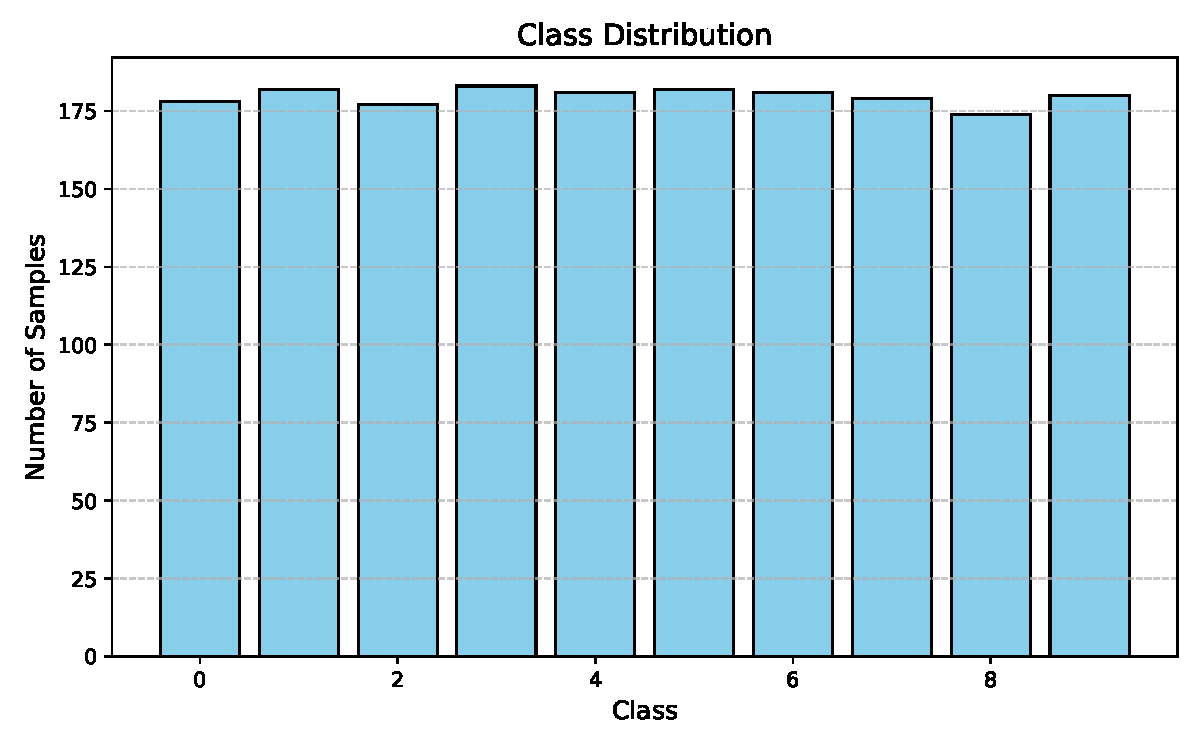
\includegraphics[width=\textwidth]{images/class_distribution.pdf}
        \caption{Class Distribution Visualization}
        \label{fig:class_distribution}
    \end{subfigure}
    \hfill
    \begin{subfigure}[b]{0.45\textwidth}
        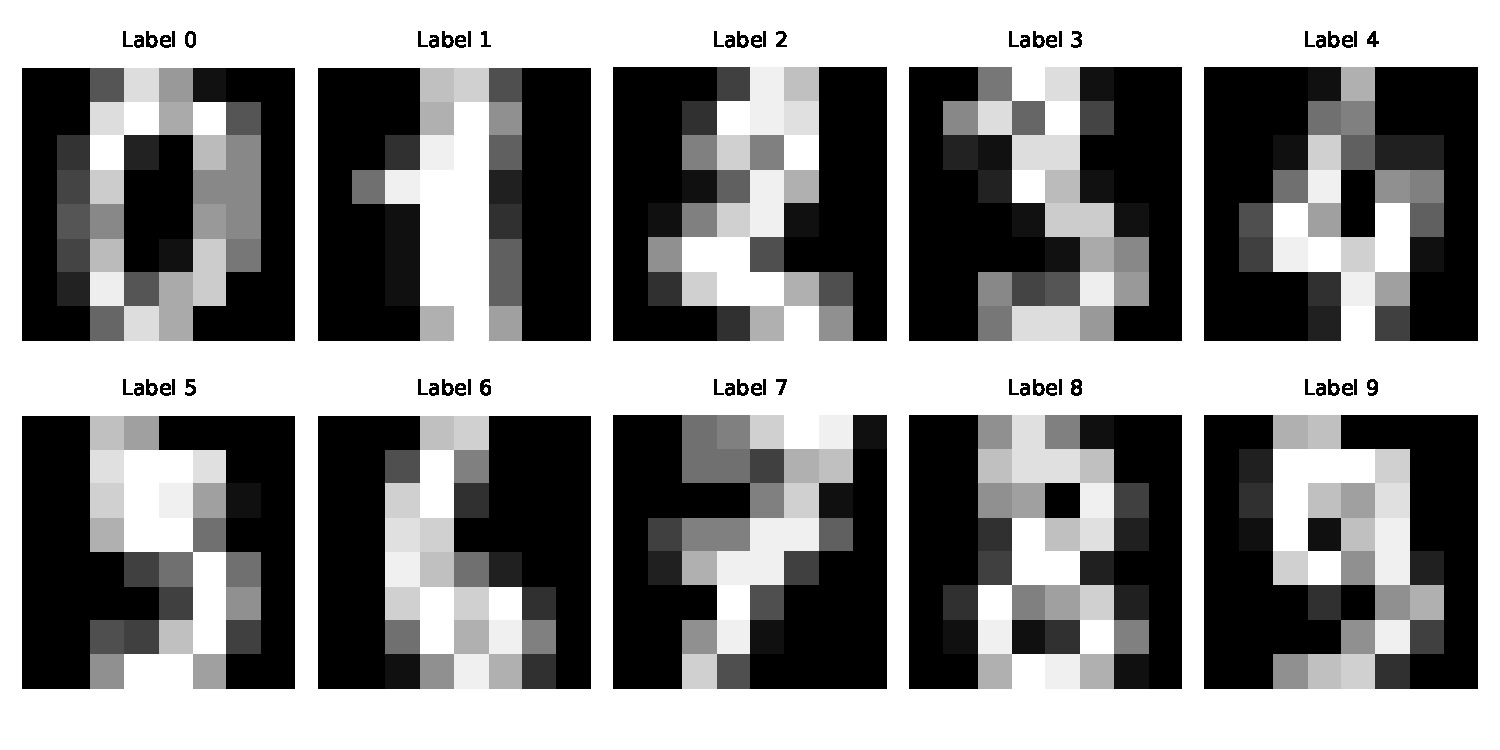
\includegraphics[width=\textwidth]{images/MNIST_samples.pdf}
        \caption{Sample MNIST Images}
        \label{fig:mnist_samples}
    \end{subfigure}
    \caption{Dataset Visualizations: Class distribution and example MNIST images.}
    \label{fig:dataset_visualizations}
\end{figure}

\subsection{Train and Test Data Split}
The dataset is split into training and test sets. The training set contains 1,437 samples, while the test set consists of 360 samples. 
The test set is reserved for evaluating the generalization performance of the trained model.

\subsection{Train and Validation Split with K-Fold Cross-Validation}
To assess model performance and mitigate overfitting, 5-fold cross-validation was applied to the training set. 
In this approach, the training data (1,437 samples) is divided into five subsets. 
For each fold, one subset is used for validation while the remaining four subsets are used for training. 

\section{Model Training and Validation}

\subsection{Model Overview}
The following machine learning models were used in this study to evaluate their robustness against data transformations.
Each model was trained with appropriate hyperparameters and settings to ensure fair evaluation.

\subsubsection{Logistic Regression}
Logistic Regression, designed for binary classification, was adapted to the multi-class task using the one-vs-rest strategy. 
The Limited-memory BFGS (LBFGS) solver was used for efficient optimization across multiple binary classifiers.

\subsubsection{Fisher Discriminant Analysis (FDA)}
Fisher Discriminant Analysis (FDA) is a linear model that finds a closed-form solution to project data onto a lower-dimensional space, maximizing class separability. 
It was employed to assess its effectiveness in handling linearly separable datasets.

\subsubsection{Support Vector Machine (SVM)}
Two variants of SVM were evaluated in this study. The first used a Gaussian kernel, a non-linear classifier effective for capturing complex decision boundaries. 
The second employed a polynomial kernel of degree 3, enabling it to model interactions between features.


\subsubsection{Multilayer Perceptron (MLP)}
The MLP model is a feedforward neural network with three hidden layers containing 128, 64, and 32 units, respectively, each using the ReLU activation function. The output layer consists of 10 units with a softmax activation function for multi-class classification. 
The model was trained using the Adam optimizer with a learning rate of 0.001 and L2 regularization ($\alpha = 10^{-4}$) to prevent overfitting, with the maximum number of optimization iterations set to 1500.

\subsubsection{Convolutional Neural Network (CNN)}
The CNN used in this study is designed for image data and features the following architecture:
\begin{enumerate}
    \item Two convolutional layers, each with 64 filters, a $3 \times 3$ kernel, and ReLU activation. Batch normalization is applied to stabilize training.
    \item A max-pooling layer with a $2 \times 2$ window for down-sampling.
    \item Two additional convolutional layers, each with 128 filters, a $3 \times 3$ kernel, and ReLU activation.
    \item A second max-pooling layer with the same configuration as the first.
    \item A fully connected layer with 256 units, followed by the output layer with 10 units, representing the classification classes.
\end{enumerate}

The model was optimized using the Adam optimizer and trained for 20 epochs with a batch size of 32.

\subsection{Validation Accuracy for Each Model}
The table below presents the average validation accuracy for each model. Overall, all models demonstrated high accuracy, reflecting their ability to effectively classify the dataset. Non-linear models and neural networks slightly outperformed linear models, but the differences in performance were not substantial.

\begin{table}[h]
    \centering
    \caption{Average Validation Accuracy for Each Model}
    \label{tab:validation_accuracy}
    \begin{tabular}{l c}
        \toprule
        \textbf{Model} & \textbf{Average Validation Accuracy} \\ 
        \midrule
        Logistic Regression & 0.9617 \\ 
        Fisher Discriminant Analysis (FDA) & 0.9478 \\ 
        SVM (Gaussian Kernel) & 0.9861 \\ 
        SVM (Polynomial Kernel) & 0.9882 \\ 
        Multilayer Perceptron (MLP) & 0.9763 \\ 
        Convolutional Neural Network (CNN) & 0.9792 \\ 
        \bottomrule
    \end{tabular}
\end{table}

\section{Experimental Setup}

\subsection{Homography Transformation}
Homography transformations were applied to simulate perspective distortions by randomly shifting the coordinates of the image corners. The maximum offset (\textit{max\_offset}) used to define the range of these random shifts was tested at three levels: 1.5, 2.0, and 2.5 pixels. These progressively severe transformations were designed to evaluate the models' ability to handle perspective changes.

\subsection{Gaussian Noise}
Gaussian noise was added to the images to simulate noisy conditions, commonly encountered in practical scenarios like low-light environments. Noise levels were defined by the standard deviation (\textit{sigma}) of the Gaussian distribution, with three levels tested: 0.2, 0.5, and 0.7. These levels introduced increasing degrees of image degradation to test the robustness of the models.

\begin{figure}[h!]
    \centering
    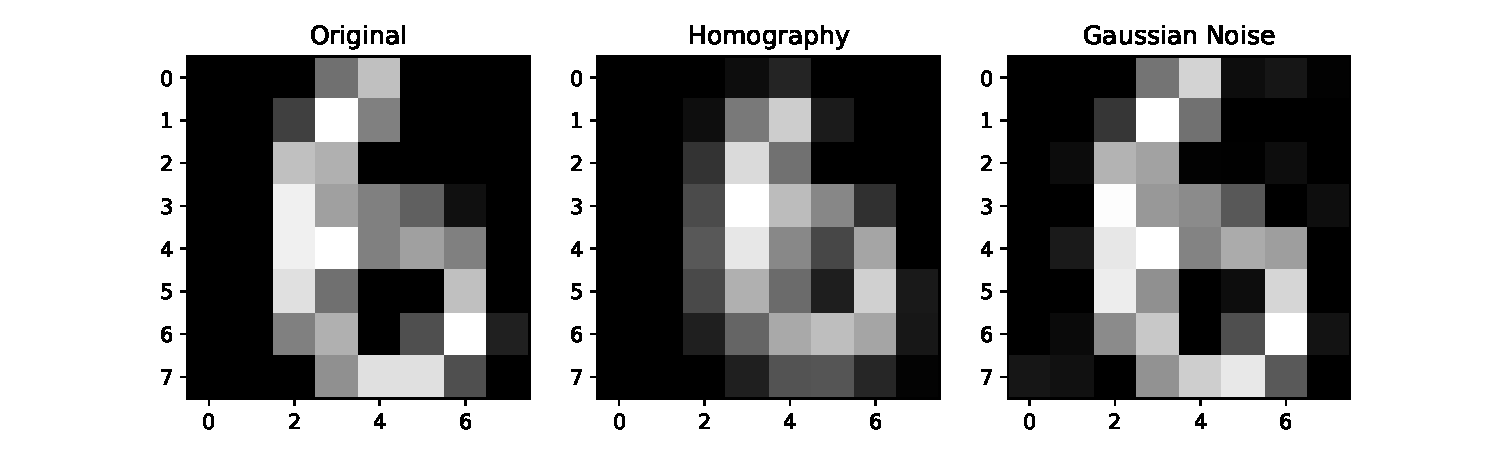
\includegraphics[width=0.8\textwidth]{images/Experiment.pdf}
    \caption{Visualization of Homography Transformation (max\_offset = 2.5) and Gaussian Noise (sigma = 0.7).}
    \label{fig:experiment_visualization}
\end{figure}

\section{Experiment Results}

\subsection{Baseline Accuracy}
The baseline accuracy represents the performance of each model on the unaltered MNIST dataset. Table~\ref{tab:baseline_accuracy} summarizes the accuracy for all models, showing that CNN and SVM with a Polynomial Kernel achieved the highest accuracy. Linear models, such as Logistic Regression and FDA, performed well but were slightly outperformed by non-linear models and neural networks.

\begin{table}[h!]
    \centering
    \caption{Baseline Accuracy for Each Model}
    \label{tab:baseline_accuracy}
    \begin{tabular}{|l|c|}
        \hline
        \textbf{Model} & \textbf{Baseline Accuracy} \\ 
        \hline
        Logistic Regression & 0.9667 \\ 
        Fisher Discriminant Analysis (FDA) & 0.9444 \\ 
        SVM (Gaussian Kernel) & 0.9861 \\ 
        SVM (Polynomial Kernel) & 0.9917 \\ 
        Multilayer Perceptron (MLP) & 0.9778 \\ 
        Convolutional Neural Network (CNN) & 0.9944 \\ 
        \hline
    \end{tabular}
\end{table}

\subsection{Homography Transformation}
For transformations with \textit{max\_offset} = 1.5, the accuracy of most models remained consistent with baseline results. As such, detailed results for this case are omitted, and the focus is on higher severity levels (\textit{max\_offset} = 2 and 2.5). 

\begin{figure}[h!]
    \centering
    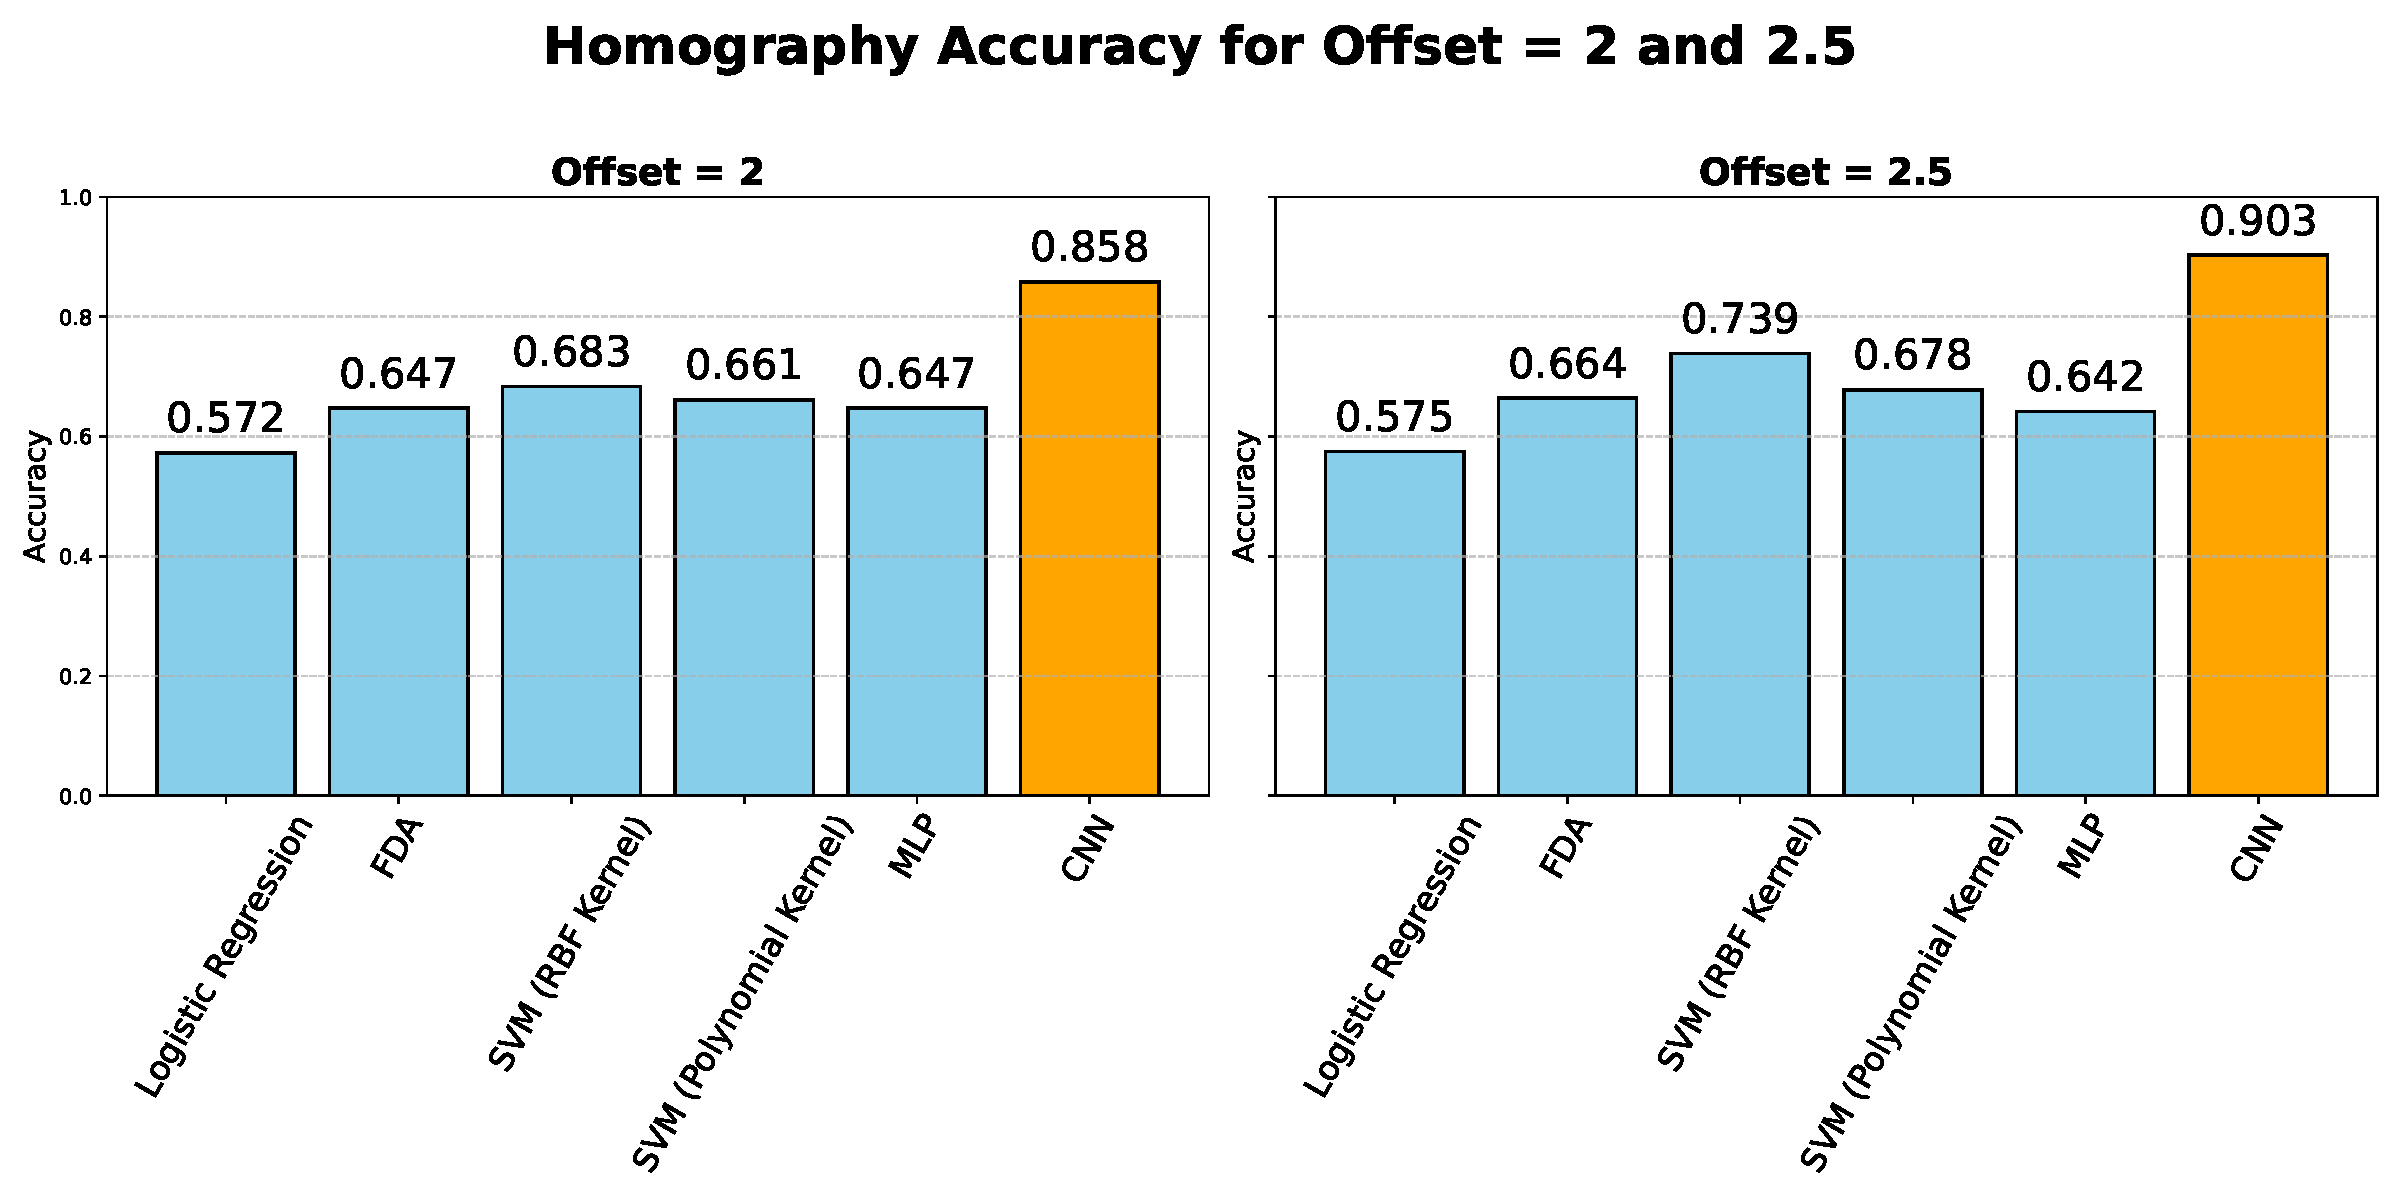
\includegraphics[width=0.8\textwidth]{images/homography.pdf}
    \caption{Accuracy under homography transformations with different max\_offset values.}
    \label{fig:homography_accuracy}
\end{figure}

\textbf{Analysis}:  
CNN displayed remarkable resilience to homography transformations, maintaining accuracy above 85\% even at \textit{max\_offset} = 2.5, leveraging its translation invariance capabilities. 
This robustness stems from CNN's ability to learn spatially invariant features through convolutional filters, making it particularly well-suited for handling geometric transformations. 
In contrast, MLP suffered as it primarily captures global patterns in the trained images, which become harder to discern under severe perspective distortions. 
SVM with a Gaussian Kernel also exhibited robust performance, benefiting from the kernel trick, which effectively increases the dimensionality of the dataset to enhance linear 
separability, as demonstrated by Cover's theorem. This capacity to handle non-linear transformations allowed SVM to maintain relatively stable accuracy despite increasing transformation severity. 
Logistic Regression experienced significant accuracy drops as the severity of the transformation increased, reflecting its limitation as a linear model incapable of modeling 
complex patterns introduced by homography. Similarly, FDA, which relies on linear assumptions, performed poorly under severe transformations. 
This method seeks to maximize class separability by projecting data onto a lower-dimensional subspace where class variance is maximized and within-class variance is minimized. 
However, the severe distortions introduced by homography transformations disrupt the relative positions and structures of the data points. 
As a result, FDA struggles to create a meaningful projection that preserves class separability, leading to a significant decline in performance.

\subsection{Gaussian Noise Transformation}
For noise levels with \textit{sigma} = 0.2, most models performed similarly to their baseline accuracy, indicating minimal impact. Results for this case are not presented, and the analysis emphasizes higher severity levels (\textit{sigma} = 0.5 and 0.7).

\begin{figure}[h!]
    \centering
    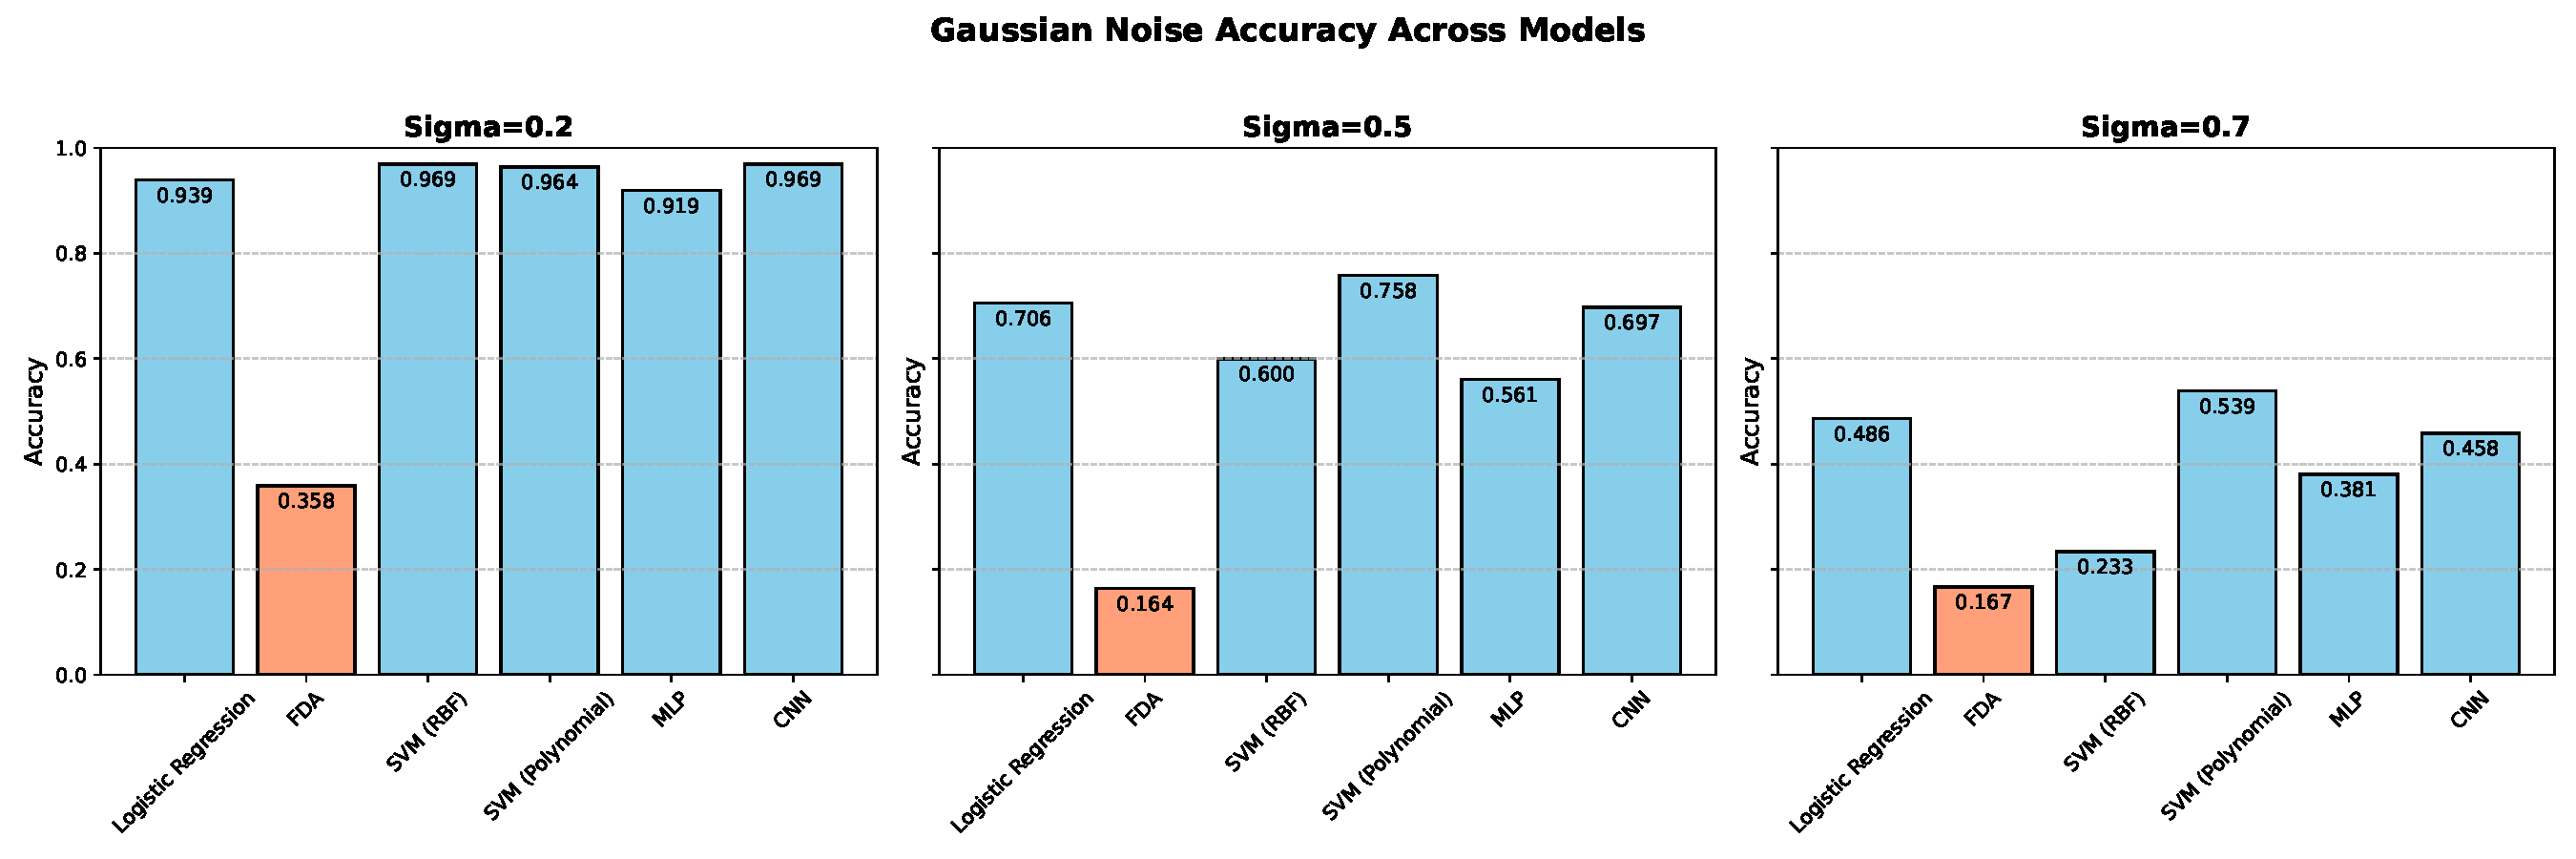
\includegraphics[width=0.8\textwidth]{images/gaussian_noise.pdf}
    \caption{Accuracy under Gaussian noise transformations with different sigma values.}
    \label{fig:gaussian_noise_accuracy}
\end{figure}

\textbf{Analysis}:  
SVM with a Polynomial Kernel demonstrated the highest tolerance to noise, particularly at \textit{sigma} = 0.5, while CNN showed moderate robustness but experienced significant degradation at \textit{sigma} = 0.7. This decline in CNN performance can be attributed to its reliance on local pattern recognition; as noise increases, the model struggles to identify these local patterns effectively. Similarly, MLP faced challenges due to its difficulty in capturing global patterns under noisy conditions. 
In contrast, Logistic Regression and SVM exhibited relatively stable performance. Logistic Regression's simplicity and reliance on linear boundaries allowed it to perform adequately at lower noise levels, as it is less influenced by distortions in the input space. SVM's robustness can be explained by its ability to transform data into higher-dimensional spaces using kernel functions, which enhances its capacity to separate classes even in noisy environments.
FDA, however, exhibited the sharpest accuracy decline, reflecting its vulnerability to noise. FDA aims to maximize the separation between classes by increasing the inter-class variance while minimizing intra-class variance. With added noise, the distinction between classes becomes blurred, making it increasingly difficult for the model to preserve inter-class variance during the dimensionality reduction process. This limitation results in a significant drop in classification accuracy under noisy conditions.

\section{Conclusion}

This study evaluated six machine learning models—Logistic Regression, FDA, SVM (Gaussian and Polynomial kernels), MLP, and CNN—under homography and Gaussian noise transformations. 
CNN handled perspective distortions best, while SVM with a Polynomial Kernel excelled in noisy conditions. 
Linear models (Logistic Regression and FDA) and MLP struggled with significant distortions. These results underscore the importance of selecting models based on robustness to specific data distortions, 
with future studies exploring diverse datasets and transformations.
\end{document}

